\documentclass[12pt]{article}

\usepackage[margin=1in]{geometry}
\usepackage{amsmath,amsthm,amssymb}
\usepackage{graphicx}

\newcommand{\N}{\mathbb{N}}
\newcommand{\Z}{\mathbb{Z}}

\newenvironment{theorem}[2][Theorem]{\begin{trivlist}
\item[\hskip \labelsep {\bfseries #1}\hskip \labelsep {\bfseries #2.}]}{\end{trivlist}}
\newenvironment{lemma}[2][Lemma]{\begin{trivlist}
\item[\hskip \labelsep {\bfseries #1}\hskip \labelsep {\bfseries #2.}]}{\end{trivlist}}
\newenvironment{exercise}[2][Exercise]{\begin{trivlist}
\item[\hskip \labelsep {\bfseries #1}\hskip \labelsep {\bfseries #2.}]}{\end{trivlist}}
\newenvironment{problem}[2][Problem]{\begin{trivlist}
\item[\hskip \labelsep {\bfseries #1}\hskip \labelsep {\bfseries #2.}]}{\end{trivlist}}
\newenvironment{question}[2][Question]{\begin{trivlist}
\item[\hskip \labelsep {\bfseries #1}\hskip \labelsep {\bfseries #2.}]}{\end{trivlist}}
\newenvironment{corollary}[2][Corollary]{\begin{trivlist}
\item[\hskip \labelsep {\bfseries #1}\hskip \labelsep {\bfseries #2.}]}{\end{trivlist}}

\newenvironment{solution}{\begin{proof}[Solution]}{\end{proof}}

\begin{document}

\title{Review Questions 2}
\author{Harald Ng \\
        Chuan Su}

\maketitle
\begin{enumerate}
\item The \texttt{map} function emits each word length plus an associated count of occurence \texttt{1}. The \texttt{reduce} function sums together all counts emiiteed for a particular word length.

\begin{verbatim}
    map(k, v) = {
        // k: blog name, the key is not used.
        // v: blog content
        for each word w in v:
          EmitIntermediate(w.length, 1);
    }
    reduce(k, vals) = {
        // k: a word
        // value: a list of counts
        result = 0
        for each v in vals:
          result += v
        emit(result)
    }
\end{verbatim}

\item Reduce-side join is used for when joining large datasets together. The different datasets will be mapped separately on each node. After shuffle and sort, the data will be joined in the reducer. Map-side join is used for when the datasets are small enough to cache. Each node will cache the data and perform the join in the mapper. Hence, the reduce phase is not performed in Map-side join.

\item The code does not work because the output of the \texttt{println} will be written to the executors' standard output instead of the driver's. Hence, we need to collect the RDD to the driver node before printing it. So to fix it, we need to change the second line to \texttt{uni.collect().foreach(println)}

\item A Spark executor is a JVM process running on a worker node, which internally uses a block manager to manage its cached data splits. If a task fails and a split is lost, Spark traces back the task lineage until cached data or the data source is found, and then it schedules recomputation tasks to recover the data.

  \begin{figure}
    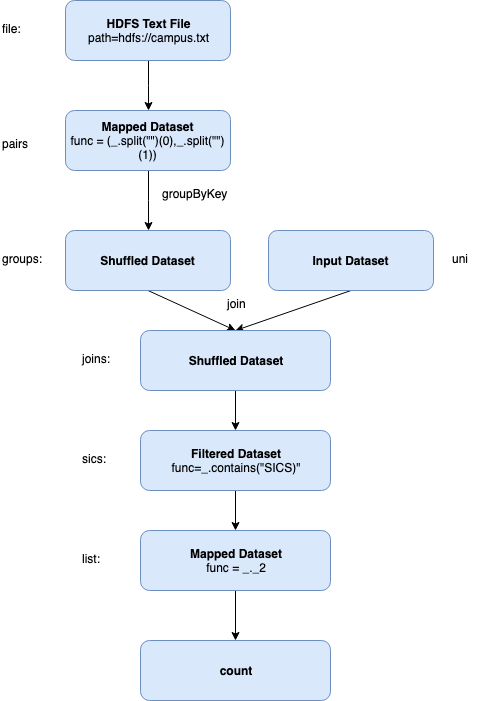
\includegraphics[width=\linewidth]{lineage_graph.png}
    \caption{Lineage Graph.}
    \label{fig:lineage_graph}
  \end{figure}

\end{enumerate}
\end{document}
